% 定常迭代法：矩阵分裂、Richardson、Jacobi、Gauss--Seidel、SOR、SSOR与停止准则
\section{定常迭代法}
\label{sec:ls-stationary-iterations}

直接法要存储并计算分解因子，矩阵很大而稀疏时，消元产生的填充会使这笔代价难以承受。本节对可逆方阵$\bm A\in\mathbb R^{d\times d}$换一条路线：用一个容易求解的矩阵近似$\bm A$，每轮根据当前残差修正近似解，每轮只需矩阵乘向量或一次三角求解。第~\ref{sec:ls-convergence}节已经建立固定更新$\bm x\mapsto\bm T\bm x+\bm c$的收敛判据，本节据此选择修正规则。下面先写清各方法共用的输入、超参数、内部状态和终止条件，再分别给出各方法的修正公式。

\subsection{矩阵分裂与定常迭代}
\label{sec:ls-matrix-splitting}

\subsubsection{主要思想}

核心做法是选一个固定、可逆且容易求解的矩阵$\bm M$，用它把当前残差$\bm r_k=\bm b-\bm A\bm x_k$转成修正量：解$\bm M\bm\delta_k=\bm r_k$，再令$\bm x_{k+1}=\bm x_k+\bm\delta_k$。若$\bm M=\bm A$，一步就得到精确解，但这要解原方程；$\bm M$只近似$\bm A$时，修正不完全准确，却便宜得多，反复修正便可逐步逼近解。记$\bm N=\bm M-\bm A$，得到矩阵分裂（matrix splitting）$\bm A=\bm M-\bm N$，上述更新与$\bm M\bm x_{k+1}=\bm N\bm x_k+\bm b$等价，因为两式都等于$\bm M\bm x_{k+1}=\bm M\bm x_k+\bm r_k$。实际执行的是对$\bm M$的求解，不形成$\bm M^{-1}$；$\bm M$不随轮次变化，所以称为定常迭代（stationary iteration）。

\subsubsection{算法实现}

\paragraph{初始化}
算法的输入为$\bm A$和$\bm b$，输出为近似解$\bm x$。超参数单独列出：初值$\bm x_0$，绝对容差$\mathrm{atol}\geq0$与相对容差$\mathrm{rtol}\geq0$，最大迭代次数$K$，以及各方法自己的固定参数。计算中保存当前解$\bm x_k$、残差$\bm r_k$和本轮修正量$\bm\delta_k$。初始化时计算$\bm r_0=\bm b-\bm A\bm x_0$，并令停止阈值$\tau=\mathrm{atol}+\mathrm{rtol}\lVert\bm b\rVert_2$。

\paragraph{停止检查}
每轮开始先检查是否停止：若$\lVert\bm r_k\rVert_2\leq\tau$或$k=K$，就结束并取$\bm x=\bm x_k$；否则进入本轮的修正。

\paragraph{求修正量并更新}
先求本轮修正量
\[
\bm M\bm\delta_k=\bm r_k .
\]
$\bm M$选得不同，这一步的算法也不同，下面各小节分别给出具体公式。得到修正量后更新当前解，并按原方程重新计算残差：
\[
\bm x_{k+1}=\bm x_k+\bm\delta_k ,\qquad
\bm r_{k+1}=\bm b-\bm A\bm x_{k+1},
\]
然后把$k$加一，回到停止检查。后面各方法都沿用这套状态和终止规则，只替换求$\bm\delta_k$的一步。

\paragraph{矩阵记号与贯穿例}
逐分量更新的方法要用到$\bm A$的元素，为此统一写$\bm A=\bm D+\bm L+\bm U$，其中$\bm D$是对角部分，$\bm L,\bm U$分别是严格下三角与严格上三角部分，元素保留$\bm A$中的符号；凡涉及对角除法，都要求$a_{i,i}\neq0$。各方法用同一个小例子对照。
\begin{example}[定常迭代的贯穿例]
\label{ex:ls-stationary-running-example}
取
\[
\bm A=\begin{bmatrix}4&1\\1&3\end{bmatrix},\qquad
\bm b=\begin{bmatrix}1\\2\end{bmatrix},\qquad
\bm x_0=\bm 0,
\]
精确解为$\bm x_\star=(1/11,7/11)^\top$，初始残差$\bm r_0=\bm b$。下面每种方法只算第一轮，足以看出各自更新方式的差别，不重复完整求解。
\end{example}

\subsubsection{算法分析}

\paragraph{收敛条件}
各方法是否收敛，取决于每轮把误差变成什么。令$\bm T=\bm I-\bm M^{-1}\bm A$为迭代矩阵，误差$\bm e_k=\bm x_k-\bm x_\star$；下面的定理把收敛问题归结为$\bm T$的谱半径，后面各小节只需分别估计各自的$\rho(\bm T)$。
\begin{theorem}[定常迭代的收敛判据]
\label{thm:ls-stationary-convergence}
设$\bm A$与$\bm M$可逆，$\bm x_\star$是$\bm A\bm x=\bm b$的解。按$\bm M\bm\delta_k=\bm r_k$，$\bm x_{k+1}=\bm x_k+\bm\delta_k$迭代时，误差满足
\[
\bm e_{k+1}=\bm T\bm e_k,\qquad \bm e_k=\bm T^k\bm e_0 ,
\]
且迭代对任意初值$\bm x_0$都收敛到$\bm x_\star$，当且仅当$\rho(\bm T)<1$。
\end{theorem}
\begin{proof}
由$\bm r_k=\bm b-\bm A\bm x_k=-\bm A\bm e_k$，更新式给出$\bm e_{k+1}=\bm e_k-\bm M^{-1}\bm A\bm e_k=\bm T\bm e_k$，归纳得$\bm e_k=\bm T^k\bm e_0$。更新也可写成仿射映射$\bm x\mapsto\bm T\bm x+\bm M^{-1}\bm b$；因为$\bm I-\bm T=\bm M^{-1}\bm A$可逆，它只有一个固定点，满足$\bm M^{-1}\bm A\bm x=\bm M^{-1}\bm b$，就是$\bm x_\star$。由定理~\ref{thm:ls-affine-common-limit}，从任意初值出发的轨迹都收敛到同一个向量当且仅当$\rho(\bm T)<1$，而这个共同极限只能是固定点$\bm x_\star$。
\end{proof}
算法可执行与算法收敛是两个条件：$a_{i,i}\neq0$只保证每轮能算下去，不保证$\rho(\bm T)<1$，反之亦然。

\paragraph{收敛速度}
渐近速度由$\bm T$的谱控制：由定理~\ref{thm:ls-gelfand-formula}，$\lVert\bm T^k\rVert^{1/k}\to\rho(\bm T)$，误差每缩小十倍约需$1/\log_{10}(1/\rho(\bm T))$轮；非正规的$\bm T$还可能在衰减前暂时放大误差（第~\ref{sec:ls-convergence-rate-transient}节）。

\subsection{Richardson迭代}
\label{sec:ls-richardson}

\subsubsection{主要思想}

Richardson迭代沿残差方向按固定比例修正当前解：残差指出哪些方程还没满足，把它乘一个步长加到解上，就朝减小残差的方向走了一步。超参数是非零步长$\alpha$，对应$\bm M=\alpha^{-1}\bm I$。方法只需要能计算$\bm A\bm v$，不必读取矩阵元素。

\subsubsection{算法实现}

内部状态沿用$\bm x_k,\bm r_k,\bm\delta_k$。每轮通过开头的检查后计算
\[
\bm\delta_k=\alpha\bm r_k,\qquad
\bm x_{k+1}=\bm x_k+\bm\delta_k,\qquad
\bm r_{k+1}=\bm b-\bm A\bm x_{k+1},
\]
然后按第~\ref{sec:ls-matrix-splitting}节的条件决定停止或继续。重算的残差同时用于检查和下一轮修正，所以每轮只需一次矩阵乘向量。贯穿例取$\alpha=1/4$，第一轮得到$\bm x_1=\tfrac14(1,2)^\top=(1/4,1/2)^\top$。

\subsubsection{算法分析}

\paragraph{收敛条件与最优步长}
此时$\bm T=\bm I-\alpha\bm A$。当$\bm A$实对称正定时，由定理~\ref{thm:ls-stationary-convergence}，收敛条件和最优步长都可以从$\bm A$的特征值直接读出。
\begin{theorem}[对称正定矩阵的Richardson迭代]
\label{thm:ls-richardson-spd}
设$\bm A$实对称正定，特征值落在$[\lambda_{\min},\lambda_{\max}]$中且两端取到。Richardson迭代对所有初值收敛当且仅当$0<\alpha<2/\lambda_{\max}$；最优固定步长为$\alpha_\star=2/(\lambda_{\min}+\lambda_{\max})$，对应的收缩因子为
\[
\rho(\bm T)=\frac{\kappa_2(\bm A)-1}{\kappa_2(\bm A)+1}.
\]
\end{theorem}
\begin{proof}
把误差按$\bm A$的标准正交特征基展开，一轮后第$i$个系数乘以$1-\alpha\lambda_i$，所以$\rho(\bm T)=\max_i|1-\alpha\lambda_i|$。它小于一当且仅当每个$\alpha\lambda_i\in(0,2)$，即$0<\alpha<2/\lambda_{\max}$。$|1-\alpha\lambda|$在区间端点取最大，$\alpha$增大时$|1-\alpha\lambda_{\min}|$变小而$|1-\alpha\lambda_{\max}|$变大，两者相等时最大值最小，即$1-\alpha\lambda_{\min}=\alpha\lambda_{\max}-1$，解得$\alpha_\star$，代回得$(\lambda_{\max}-\lambda_{\min})/(\lambda_{\max}+\lambda_{\min})$，再用$\kappa_2(\bm A)=\lambda_{\max}/\lambda_{\min}$。
\end{proof}
\paragraph{收敛速度与代价}
谱范围越宽，$\kappa_2(\bm A)$越大，收缩因子越接近一，收敛越慢。每轮的主要代价是一次矩阵乘向量，约$2\operatorname{nnz}(\bm A)$次运算。实际中谱端点未知，步长按已知的谱界选取，例如用$\lVert\bm A\rVert$作$\lambda_{\max}$的上界；贯穿例的$\lambda_{\max}\approx4.618$，$\alpha=1/4$在收敛区间内。停止时的残差与解误差之间的关系在第~\ref{sec:ls-stationary-stopping}节解释。

\subsection{Jacobi迭代}
\label{sec:ls-jacobi}

\subsubsection{主要思想}

Jacobi迭代让每个方程只修正自己的对角未知量：从第$i$个方程解出$x_i$，其余分量暂取旧值。这相当于用对角矩阵近似$\bm A$，取$\bm M=\bm D$；对角元相对非对角元越大，这个近似越好。

\subsubsection{算法实现}

\paragraph{逐分量修正}
每轮在通过检查后，全部分量都由同一个旧状态$\bm x_k,\bm r_k$计算：
\[
\begin{aligned}
(\bm\delta_k)_i&=\frac{(\bm r_k)_i}{a_{i,i}},\\
(\bm x_{k+1})_i&=(\bm x_k)_i+(\bm\delta_k)_i
=\frac{b_i-\sum_{j\neq i}a_{i,j}(\bm x_k)_j}{a_{i,i}},
\end{aligned}
\qquad i=1,\ldots,d .
\]
\paragraph{整体替换}
右端求和只读旧向量$\bm x_k$，新分量写进另一个向量，全部$d$个分量算完后才替换旧向量，再计算$\bm r_{k+1}=\bm b-\bm A\bm x_{k+1}$并检查终止。若算出一个分量就覆盖旧值，后面的行会读到本轮的新值，得到的就是下一小节的Gauss--Seidel迭代。

\paragraph{加权Jacobi}
加权Jacobi迭代只增加一个固定超参数$\omega>0$，把修正改成$\bm\delta_k=\omega\bm D^{-1}\bm r_k$，其余流程不变；$\omega=1$恢复原方法。

\begin{example}[Jacobi迭代的第一轮]
\label{ex:ls-jacobi-first-sweep}
在例~\ref{ex:ls-stationary-running-example}中，$\bm x_0=\bm 0$，$\bm r_0=\bm b=(1,2)^\top$。两个分量都用这个旧残差除以各自的对角元：$(\bm\delta_0)_1=1/4$，$(\bm\delta_0)_2=2/3$，所以$\bm x_1=(1/4,\,2/3)^\top$。整体替换后重算残差，$\bm A\bm x_1=(5/3,\,9/4)^\top$，$\bm r_1=(-2/3,\,-1/4)^\top$，$\lVert\bm r_1\rVert_2\approx0.71$，比$\lVert\bm r_0\rVert_2\approx2.24$小。两个修正都过了头，残差变成负的：每个分量都在假定另一个分量不变的前提下修正，而另一个分量同时也在变。
\end{example}

\subsubsection{算法分析}

\paragraph{收敛条件}
Jacobi的迭代矩阵为$\bm T_{\mathrm J}=-\bm D^{-1}(\bm L+\bm U)$，第$i$行的非对角元为$-a_{i,j}/a_{i,i}$。当每行的对角元压过同一行其余元素时，这个矩阵的行和范数小于一，由此得到常用的充分条件。
\begin{theorem}[Jacobi迭代的收敛条件]
\label{thm:ls-jacobi-convergence}
若$\bm A$严格行对角占优，即每行$|a_{i,i}|>\sum_{j\neq i}|a_{i,j}|$，则
\[
q=\lVert\bm T_{\mathrm J}\rVert_\infty=\max_i\frac{\sum_{j\neq i}|a_{i,j}|}{|a_{i,i}|}<1,
\]
Jacobi迭代对所有初值收敛，且$\lVert\bm e_k\rVert_\infty\leq q^k\lVert\bm e_0\rVert_\infty$。
\end{theorem}
\begin{proof}
$\infty$-范数诱导的矩阵范数等于最大行绝对值和，$\bm T_{\mathrm J}$第$i$行的绝对值和正是$\sum_{j\neq i}|a_{i,j}|/|a_{i,i}|$，对角占优使它小于一。由定理~\ref{thm:ls-stationary-convergence}，$\bm e_k=\bm T_{\mathrm J}^k\bm e_0$，再用范数的次乘性得$\lVert\bm e_k\rVert_\infty\leq q^k\lVert\bm e_0\rVert_\infty\to0$。
\end{proof}
贯穿例中$q=1/3$。对称正定本身并不够：$\bm A=\bm I+2\bm 1\bm 1^\top\in\mathbb R^{3\times3}$的特征值为$7,1,1$，而$\bm T_{\mathrm J}=-\tfrac23(\bm 1\bm 1^\top-\bm I)$沿$\bm 1$方向的特征值为$-4/3$，$\rho(\bm T_{\mathrm J})=4/3$，迭代发散。

\paragraph{并行性与数值敏感度}
各分量的更新互不依赖，可以并行；一轮工作量与$\operatorname{nnz}(\bm A)$同阶。很小的对角元会把残差分量放大成很大的修正，也放大其中的舍入误差。

\paragraph{加权Jacobi的步长范围}
对加权Jacobi，设$\bm A$实对称正定，则$\bm D$的对角元为正，迭代矩阵$\bm I-\omega\bm D^{-1}\bm A$与$\bm I-\omega\bm D^{-1/2}\bm A\bm D^{-1/2}$相似，后者对称。按Richardson迭代的同样论证，收敛当且仅当
\[
0<\omega<\frac{2}{\lambda_{\max}(\bm D^{-1/2}\bm A\bm D^{-1/2})}.
\]
原方法对应$\omega=1$，未必位于这个区间：上例中$\bm D^{-1/2}\bm A\bm D^{-1/2}=\bm A/3$，区间为$(0,6/7)$。

\subsection{Gauss--Seidel迭代}
\label{sec:ls-gauss-seidel}

\subsubsection{主要思想}

Jacobi在计算后面的分量时，没有用到本轮已经算出的前面分量。Gauss--Seidel迭代按顺序更新，并立即使用本轮已经得到的修正，取$\bm M=\bm D+\bm L$。新信息进入得更早，修正通常更准确，代价是各行之间有了先后依赖。

\subsubsection{算法实现}

\paragraph{前代求修正量}
变量顺序作为超参数固定为$1,\ldots,d$。每轮通过检查后，依次计算
\[
(\bm\delta_k)_i=\frac{(\bm r_k)_i-\sum_{j<i}a_{i,j}(\bm\delta_k)_j}{a_{i,i}},\qquad i=1,\ldots,d .
\]
第$i$个修正只用到已经算出的前$i-1$个修正，这正是用第~\ref{sec:ls-lu}节的前代求解下三角方程$(\bm D+\bm L)\bm\delta_k=\bm r_k$。

\paragraph{更新与原位覆盖}
完成修正后令$\bm x_{k+1}=\bm x_k+\bm\delta_k$，重算$\bm r_{k+1}=\bm b-\bm A\bm x_{k+1}$并检查终止。把$(\bm r_k)_i=b_i-\sum_j a_{i,j}(\bm x_k)_j$代入上式，得到逐坐标形式
\[
(\bm x_{k+1})_i=\frac{b_i-\sum_{j<i}a_{i,j}(\bm x_{k+1})_j-\sum_{j>i}a_{i,j}(\bm x_k)_j}{a_{i,i}} ,
\]
下三角部分用的是本轮的新值，上三角部分仍用旧值；实现时直接在一个向量上原位覆盖即可。

\begin{example}[Gauss--Seidel迭代的第一轮]
\label{ex:ls-gauss-seidel-first-sweep}
仍从例~\ref{ex:ls-stationary-running-example}的$\bm x_0=\bm 0$，$\bm r_0=(1,2)^\top$出发。前代的第一行与Jacobi相同，$(\bm\delta_0)_1=1/4$；第二行扣掉刚得到的修正对它的影响，$(\bm\delta_0)_2=(2-1\cdot\tfrac14)/3=7/12$。于是$\bm x_1=(1/4,\,7/12)^\top$，重算得$\bm r_1=(-7/12,\,0)^\top$，$\lVert\bm r_1\rVert_2\approx0.58$。第二个残差分量为零，因为最后一次坐标修正恰好让第二个方程成立；与例~\ref{ex:ls-jacobi-first-sweep}的$(1/4,2/3)^\top$相比，差别正来自第二行用了新的第一分量。
\end{example}

\subsubsection{算法分析}

\paragraph{收敛条件}
迭代矩阵为$\bm T_{\mathrm{GS}}=-(\bm D+\bm L)^{-1}\bm U$。由定理~\ref{thm:ls-stationary-convergence}，只需说明$\rho(\bm T_{\mathrm{GS}})<1$；下面的定理给出两类常用的充分条件。
\begin{theorem}[Gauss--Seidel迭代的收敛条件]
\label{thm:ls-gauss-seidel-convergence}
若$\bm A$严格行对角占优，或$\bm A$实对称正定，则$\rho(\bm T_{\mathrm{GS}})<1$，Gauss--Seidel迭代对所有初值收敛。
\end{theorem}
\begin{proof}
先设严格行对角占优。若$\bm T_{\mathrm{GS}}\bm v=\lambda\bm v$，$\bm v\neq\bm 0$，$|\lambda|\geq1$，则$-\bm U\bm v=\lambda(\bm D+\bm L)\bm v$。取$|v_i|$最大的分量，第$i$行给出
\[
|a_{i,i}||v_i|\leq\sum_{j<i}|a_{i,j}||v_j|+\frac{1}{|\lambda|}\sum_{j>i}|a_{i,j}||v_j|
\leq|v_i|\sum_{j\neq i}|a_{i,j}|,
\]
与对角占优矛盾。

再设$\bm A$实对称正定，令$\phi(\bm x)=\tfrac12\bm x^\top\bm A\bm x-\bm b^\top\bm x$，则$\phi(\bm x)-\phi(\bm x_\star)=\tfrac12\bm e^\top\bm A\bm e$。沿第$i$个坐标移动$t$时，$\phi$的变化为$-t\,r_i+\tfrac12t^2a_{i,i}$，其中$r_i$是当前残差的第$i$个分量；Gauss--Seidel取$t=r_i/a_{i,i}$，使$\phi$减少$r_i^2/(2a_{i,i})\geq0$。若一整轮$\phi$没有减少，则每次$r_i=0$，各分量都没有改变，从而$\bm r_k=\bm 0$。所以对$\bm e\neq\bm 0$有$\bm e^\top\bm A\bm e>(\bm T_{\mathrm{GS}}\bm e)^\top\bm A(\bm T_{\mathrm{GS}}\bm e)$，即$\bm A-\bm T_{\mathrm{GS}}^\top\bm A\bm T_{\mathrm{GS}}$正定。用正定平方根（第~\ref{sec:ls-matrix-square-root}节）令$\bm C=\bm A^{-1/2}(\bm A-\bm T_{\mathrm{GS}}^\top\bm A\bm T_{\mathrm{GS}})\bm A^{-1/2}$，它的最小特征值$\mu\in(0,1]$与轮次无关，由Rayleigh--Ritz定理（定理~\ref{thm:matrix-analysis-rayleigh-ritz}）得一轮的统一收缩
\[
\lVert\bm e_{k+1}\rVert_{\bm A}^2\leq(1-\mu)\lVert\bm e_k\rVert_{\bm A}^2,\qquad
\lVert\bm e\rVert_{\bm A}^2=\bm e^\top\bm A\bm e ,
\]
故$\rho(\bm T_{\mathrm{GS}})\leq\sqrt{1-\mu}<1$。
\end{proof}
\paragraph{收敛速度与代价}
收敛速度取决于$\bm T_{\mathrm{GS}}$的谱，而重新排列变量会改变$\bm L,\bm U$的划分，从而改变迭代矩阵本身。一轮是一次三角扫掠，工作量与$\operatorname{nnz}(\bm A)$同阶。贯穿例中$\rho(\bm T_{\mathrm{GS}})=1/12$，小于Jacobi的$\rho(\bm T_{\mathrm J})=1/\sqrt{12}\approx0.289$，图~\ref{fig:ls-stationary-iteration-paths}画出了这一差别：左图中Gauss--Seidel的每个半步只改一个坐标，并恰好落在对应方程的直线上，折线很快收拢到$\bm x_\star$，而Jacobi的两个分量同时按旧值修正，在解的两侧来回跳动；右图的半对数坐标中，各方法的误差大致沿直线下降，斜率对应各自的谱半径。新值的复用带来了顺序依赖，却不保证对所有矩阵都比Jacobi快：有的矩阵上Jacobi收敛而Gauss--Seidel发散。

\begin{figure}[htbp]
  \centering
  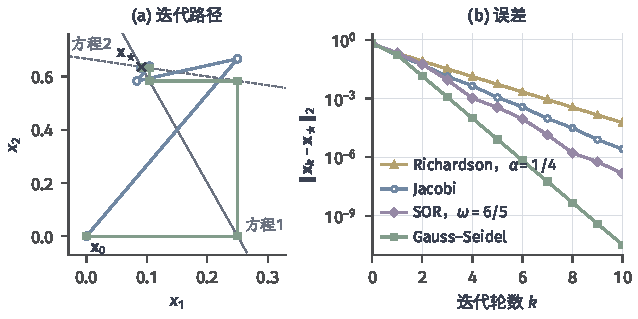
\includegraphics[width=108mm]{figures/01-basic-mathematics/03-vectors-matrices-and-multivariate-functions/matplotlib/c5-stationary-iteration-paths/figure.pdf}
  \caption{定常迭代在贯穿例$\bm A=\begin{bmatrix}4&1\\1&3\end{bmatrix}$，$\bm b=(1,2)^\top$，$\bm x_0=\bm 0$上的真实迭代值。左：实线与虚线分别是第一、第二个方程的解集，两者交于$\bm x_\star=(1/11,7/11)^\top$；蓝色圆点为Jacobi前四轮的迭代点，绿色折线为Gauss--Seidel前三轮的逐坐标路径。右：Richardson（$\alpha=1/4$）、Jacobi、SOR（$\omega=6/5$）与Gauss--Seidel的误差$\lVert\bm x_k-\bm x_\star\rVert_2$，纵轴取对数，渐近斜率分别对应谱半径约$0.40$、$0.29$、$0.20$与$1/12$。}
  \label{fig:ls-stationary-iteration-paths}
\end{figure}

\subsection{SOR迭代}
\label{sec:ls-sor}

\subsubsection{主要思想}

Gauss--Seidel每次坐标修正都恰好让当前方程成立，修正幅度是固定的。逐次超松弛迭代（successive over-relaxation，SOR）在每次坐标修正中乘一个固定的松弛参数$\omega\neq0$：$\omega>1$时放大修正，$\omega<1$时缩小修正，目的是在误差沿同一方向缓慢衰减时走得更快，或在修正过冲时收敛得更稳。

\subsubsection{算法实现}

\paragraph{松弛前代}
每轮通过检查后，按既定顺序求解$(\bm D+\omega\bm L)\bm\delta_k=\omega\bm r_k$，即
\[
(\bm\delta_k)_i=\frac{\omega}{a_{i,i}}\Bigl((\bm r_k)_i-\sum_{j<i}a_{i,j}(\bm\delta_k)_j\Bigr),\qquad i=1,\ldots,d .
\]
计算当前分量时用到的，已经是前面分量松弛后的修正；$\omega=1$时恢复Gauss--Seidel。

\paragraph{更新与检查}
随后令$\bm x_{k+1}=\bm x_k+\bm\delta_k$，重算残差并检查终止。

\begin{example}[SOR迭代的第一轮]
\label{ex:ls-sor-first-sweep}
在例~\ref{ex:ls-stationary-running-example}中取$\omega=6/5$。第一分量的修正为$\tfrac65\cdot\tfrac14=3/10$，第二分量用这个松弛后的值，修正为$\tfrac65\cdot(2-3/10)/3=17/25$，所以$\bm x_1=(3/10,\,17/25)^\top$，残差$\bm r_1=(-22/25,\,-17/50)^\top$。与例~\ref{ex:ls-gauss-seidel-first-sweep}不同，第二个方程不再恰好成立，因为它的修正被放大了五分之一。若先做完整一轮Gauss--Seidel、再把两个完整向量按$\omega$加权，得到的是$\tfrac65(1/4,7/12)^\top=(3/10,7/10)^\top$；两者不同，说明SOR的松弛发生在每个坐标内部。
\end{example}

\subsubsection{算法分析}

\paragraph{收敛条件}
SOR的迭代矩阵为
\[
\bm T_\omega=\bm I-\omega(\bm D+\omega\bm L)^{-1}\bm A=(\bm D+\omega\bm L)^{-1}\bigl[(1-\omega)\bm D-\omega\bm U\bigr].
\]
松弛参数不能随意取：它的取值范围对一般矩阵有一条必要条件，对实对称正定矩阵则恰好也是充分条件。
\begin{theorem}[SOR迭代的收敛条件]
\label{thm:ls-sor-convergence}
设$\bm A$的对角元全不为零。
\begin{enumerate}
\item 对任意这样的方阵，$\rho(\bm T_\omega)\geq|1-\omega|$；所以SOR对所有初值收敛的必要条件是$0<\omega<2$。
\item 若$\bm A$实对称正定且$0<\omega<2$，则$\rho(\bm T_\omega)<1$，SOR对所有初值收敛。
\end{enumerate}
\end{theorem}
\begin{proof}
（1）$\bm D+\omega\bm L$是下三角阵，行列式为$\prod_i a_{i,i}$；$(1-\omega)\bm D-\omega\bm U$是上三角阵，行列式为$(1-\omega)^d\prod_i a_{i,i}$。所以$\det\bm T_\omega=(1-\omega)^d$。行列式等于全部特征值之积，其模不超过$\rho(\bm T_\omega)^d$，故$\rho(\bm T_\omega)\geq|1-\omega|$。若$\omega\leq0$或$\omega\geq2$，则$\rho(\bm T_\omega)\geq1$，由定理~\ref{thm:ls-stationary-convergence}不能对所有初值收敛。

（2）第$i$次坐标修正的步长是$t=\omega r_i/a_{i,i}$，代入定理~\ref{thm:ls-gauss-seidel-convergence}证明中的能量变化式，$\phi$减少$\omega(2-\omega)r_i^2/(2a_{i,i})$。当$0<\omega<2$时这是非负量，且只在$r_i=0$时为零，此后的统一收缩论证与该证明相同。
\end{proof}

\paragraph{参数选择与代价}
收敛速度取决于参数和变量排列：三对角等特殊结构的矩阵有由$\rho(\bm T_{\mathrm J})$给出的最优参数公式，但不能普遍套用，贯穿例的$\omega=6/5$就使谱半径从Gauss--Seidel的$1/12$升到$0.2$。一轮成本与Gauss--Seidel同阶；$\omega$接近区间端点时收缩因子接近一，收敛可能很弱。

\subsection{SSOR迭代}
\label{sec:ls-ssor}

\subsubsection{主要思想}

单向扫掠依赖变量顺序，对应的$\bm M$也不对称。对实对称正定的$\bm A$，对称逐次超松弛迭代（symmetric SOR，SSOR）把一次前向SOR扫掠与一次反向SOR扫掠配成一轮，超参数取固定的$0<\omega<2$。两次扫掠合起来对应的修正矩阵为
\[
\bm M_{\mathrm{SSOR}}=\frac{1}{\omega(2-\omega)}(\bm D+\omega\bm L)\bm D^{-1}(\bm D+\omega\bm U),
\]
它对称正定，这使SSOR除了单独迭代，还能为第~\ref{sec:ls-krylov-iterations}节的方法提供预条件。

\subsubsection{算法实现}

内部状态除$\bm x_k,\bm r_k,\bm\delta_k$外，只多一个本轮的中间向量$\bm y_k$。下面直接按$\bm M_{\mathrm{SSOR}}$的三个因子求修正量。

\paragraph{前代求中间向量}
第一步，用第~\ref{sec:ls-lu}节的前代求解
\[
(\bm D+\omega\bm L)\bm y_k=\bm r_k ,
\]
得到本轮的中间向量$\bm y_k$。

\paragraph{缩放后回代}
然后把中间向量按对角元缩放，再用回代求解上三角方程
\[
(\bm D+\omega\bm U)\bm\delta_k=\omega(2-\omega)\bm D\bm y_k .
\]
依次代入可知，所得$\bm\delta_k$正是$\bm M_{\mathrm{SSOR}}\bm\delta_k=\bm r_k$的解。

\paragraph{更新与检查}
最后更新$\bm x_{k+1}=\bm x_k+\bm\delta_k$，重算$\bm r_{k+1}=\bm b-\bm A\bm x_{k+1}$并检查终止。贯穿例取$\omega=1$：前代得$\bm y_0=(1/4,\,7/12)^\top$，缩放后右端为$\bm D\bm y_0=(1,\,7/4)^\top$，回代先得第二分量$7/12$、再得第一分量$(1-7/12)/4=5/48$，整轮得到$\bm x_1=(5/48,\,7/12)^\top$。

\subsubsection{算法分析}

\paragraph{对称正定性与扫掠的等价}
由$\bm U=\bm L^\top$，令$\bm F=(\bm D+\omega\bm L)\bm D^{-1/2}$，则$\bm M_{\mathrm{SSOR}}=\bm F\bm F^\top/(\omega(2-\omega))$，$\bm F$可逆且系数为正，所以$\bm M_{\mathrm{SSOR}}$对称正定。把前向扫掠$\bm x_k+\omega(\bm D+\omega\bm L)^{-1}\bm r_k$与随后的反向扫掠合并，并用$(\bm D+\omega\bm L)+(\bm D+\omega\bm U)-\omega\bm A=(2-\omega)\bm D$化简，恰好得到$\bm M_{\mathrm{SSOR}}^{-1}\bm r_k$，所以按因子求解与两次逐坐标扫掠是同一个更新。

\paragraph{收敛性与代价}
两次扫掠中的每一步都是SOR的坐标修正，能量下降不依赖顺序，定理~\ref{thm:ls-sor-convergence}第二部分的统一收缩论证照样成立，SSOR对所有初值收敛；速度由整轮误差矩阵$\bm I-\bm M_{\mathrm{SSOR}}^{-1}\bm A$的谱决定。每轮含两次扫掠，代价约为SOR的两倍，比较时不能只数轮数。便于求解的对称正定因子还可以在第~\ref{sec:ls-preconditioning}节作为预条件使用。

\subsection{收敛检验与停止准则}
\label{sec:ls-stationary-stopping}

各方法都使用第~\ref{sec:ls-matrix-splitting}节的终止条件：$\lVert\bm r_k\rVert_2\leq\mathrm{atol}+\mathrm{rtol}\lVert\bm b\rVert_2$，或$k=K$。前者表示达到了给定的残差要求；后者只表示不再继续计算，结果未必达到精度。两种情况下输出都只有当前的$\bm x_k$。残差与修正量是内部计算量，不追加到输出；修正量$\lVert\bm\delta_k\rVert$很小也不能代替原方程的残差检验，因为收缩因子接近一时，步长很小可能只说明迭代很慢。

残差小也不等于解的误差小。由$\bm x_\star-\bm x_k=\bm A^{-1}\bm r_k$，误差是残差经$\bm A^{-1}$放大的结果，两者之间隔着问题本身的敏感性；第~\ref{sec:ls-numerical-sensitivity}节再给出误差界和后向误差的解释。比较不同方法时，应在相同精度要求下比较总工作量，而不是轮数；分析中的收敛率和代价用于解释算法，不加入求解器的输出。其他用递推方式维护残差的方法，递推值会因舍入而偏离真实残差，停止前也须用$\bm b-\bm A\bm x_k$复核。
